%!TEX root = ../thesis.tex
%*******************************************************************************
%****************************** Third Chapter **********************************
%*******************************************************************************
\chapter{Approach}
\graphicspath{{Chapter3/Figs/Raster/}{Chapter3/Figs/}}

\section{Scope}

The aim of this project focuses on improving assessments and curriculum personalisation, and does not require 
coverage of all elements in the Learning Technology Systems Architecture (LTSA, Chapter 2.2.1). 
See Figure \ref{fig:ltsa-covered} for which parts of LTSA this project will attempt to cover, and 
Table \ref{table:ltsa-bcu} for the mappings from LTSA elements to the blockchain design objects in this project.

Components such as delivery and the storage of learning resources will be out of the scope of this project. 
A blockchain is also not the ideal storage service for multimedia data such as learning content and delivery activities 
due to the inherent high latency in consensus. Security and redundancy of these data is also unnecessary. 

\begin{figure}[!ht] 
    \centering    
    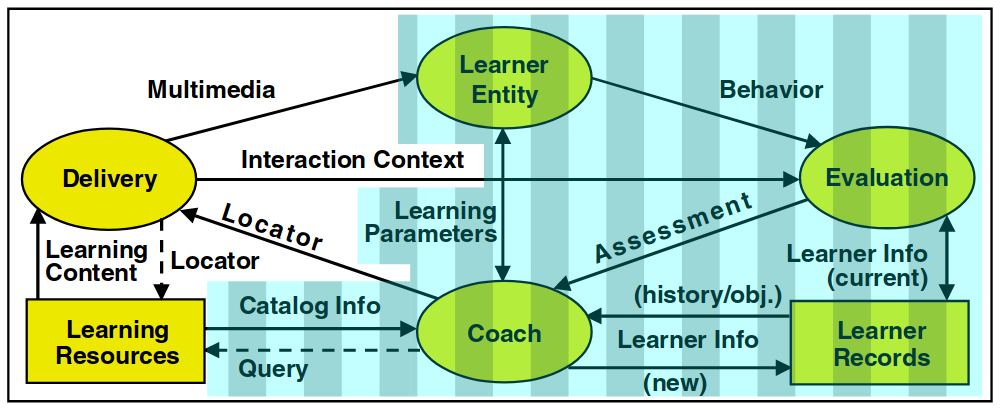
\includegraphics[width=0.85\textwidth]{ltsa-covered}
    \caption[Design Coverage of LTSA]
        {The Learning Technology Systems Architecture \citep{ieee2003ltsa}, 
        with components covered by this project highlighted in cyan} 
    \label{fig:ltsa-covered}
\end{figure}

\begin{table}[!h] 
    \caption{Mappings between LTSA elements and the BlockChain objects in this project}
    \centering
    \label{table:ltsa-bcu}
    \begin{tabularx}{\textwidth}{l|X}
        \textbf{LTSA Elements} & \textbf{BlockChain Objects}
        \\\toprule
        Learner Entity (component) & Learner
        \\\midrule
        Coach (component) & Teacher
        \\\midrule
        Evaluation (component) & Assessment Results, Feedback
        \\\midrule
        Behavior (flow) & Submission
        \\\midrule
        Catalog Info (flow) & Course Modules, Module Units
        \\\midrule
        Assessment (flow) & Assessment (Automatic Assessment, Assessor Assessment, etc.)
        \\\midrule
        Learner Info (flow) & Curriculum (a collection of Course Modules)
        \\\midrule
        Learning Parameters (flow) & Negotiation
        \\\midrule
        Learner Records (component) & Certificates, Submission, Assessment Results
        \\\bottomrule
    \end{tabularx}
\end{table}

\section{Project Timeline}

\begin{figure}[!hb] 
    \centering    
    \includegraphics[width=1.0\textwidth]{simple_gantt}
    \caption[Project Timeline]
        {A timeline of the stages of actions in this project and their dependencies if any, loosely based on a Gantt chart} 
    \label{fig:simple_gantt}
\end{figure}

Figure \ref{fig:simple_gantt} shows the ten main stages of action, their timeframe and dependencies.
Fairly waterfall... research specific?

\section{Agile Software Development}

% \begin{figure}[!hb] 
%     \centering    
%     \includegraphics[width=1.0\textwidth]{}
%     \caption[Extreme Programming]
%         {A timeline of the stages of actions in this project and their dependencies if any, loosely based on a Gantt chart} 
%     \label{fig:}
% \end{figure}

There are some agile software development principles that this project has chosen to adopt. 
Some clear limitations exist, for example, \citet{beck2001agile}'s agile manifesto asks for 
daily collaboration between customer and developers, and teamwork and interactions

Here are the tools that this project has used to manage the agile process. Here is 

Trello as Kanban

Github is a git-based version control, code hosting and project management service that offers free 
private repositories to verified students \citep{github2018education}.

\begin{figure}[!hb] 
    \centering    
    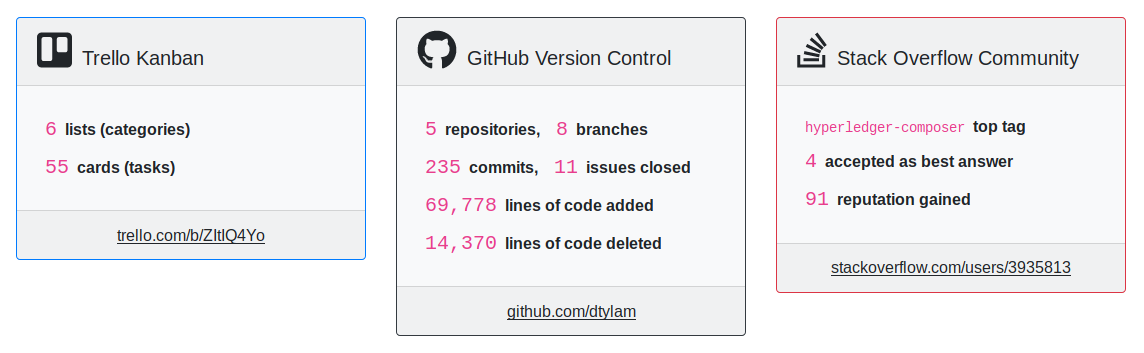
\includegraphics[width=1.0\textwidth]{platforms_stats}
    \caption[Project Management Statistics]
        {Statistics from Trello, GitHub and Stack Overflow collected over the duration of this project} 
    \label{fig:platforms_stats}
\end{figure}

% \section{ and Testing}

